\chapter{Introduction}
\label{cha:intro}


% SECTION 1

\section{Microbial communities: composition 
% (\textit{who})
, functions 
% (\textit{what}) 
\& intections 
% (\textit{how})
}


   % WHO : DIVERSITY 
   % \if 0
   \subsection{Microbial diversity}
   % \fi
   Microbes are considered to be omnipresent in the 
   various ecosystems on Earth~\citep{falkowski2008microbial}.
   It was only until recently, \citeyear{belilla2019hyperdiverse}, that scientists discovered for the first time 
   a place on Earth where no microbial forms of life are present~\cite{belilla2019hyperdiverse}.
   Extremely low pH, high salt and high temperature had to be 
   at the same place at the same time to stop microbes.
   However, microbes are not just abundant but 
   exceedingly variant too.
   \citeauthor{locey2016scaling} using a unified scaling law
   and a lognormal model of biodiversity, 
   estimated microbial diversity at about 1 trillion species~\cite{locey2016scaling}.
   However, despite the extensive studies of the scientific community, 
   less than 1\% of the microbial species on Earth have been identified~\cite{isme}.
   
   Microbes are distinguished by multiple properties.
   Based on their morphology microbes can be spherical (cocci), rod-shaped (bacilli),
   arc-shaped (vibrio), and spiral (spirochete)~\cite{dunlap2001microbial}.
   Based on their metabolic characteristics, microbes are further distinguished. 
   More specifically, according to their \textit{energy source}, a microbe
   can either oxidate inorganic compounds (\textbf{chemotrophs}) or sunlight (\textbf{phototrophs}).
   Similarly, microbes can use CO$_2$ (\textbf{autotrophs}) as their \textit{carbon source},
   or organic compounds (\textbf{heterotrophs}) or both (\textbf{mixotrophs}).
   Finally, based on their \textit{electron source} 
   microbes are distinguished bewtween those using inorgarnic compounds (\textbf{lithotrophs}) and those using organic compounds (\textbf{organotrophs})~\cite{madigan2018brock}.
   Microbial taxa combine combinining alternatives of the aforementioned categories 
   shape a range of microbial profile of all the possible combinations; for example      \textbf{chemolithoautotrophic} bacteria, 
   e.g. nitrifying and sulfur-oxidizing bacteria, as well
   as \textbf{photoautotrophic} bacteria, 
   e.g. purple bacteria and Green sulfur bacteria. 
   Finally, microbia taxa can also be disinguished by their various ecological distributions and activities, 
   and by their distinct genomic structure, expression, and evolution~\cite{dunlap2001microbial}. 

   % WHAT : FUNCTIONAL POTENTIAL
   % \if 0
   \subsection{Functional diversity and contribution}
   % \fi 
   However, it is not only the number of microbial taxa and their massive biomass that
   make the study of microbial communities essential; 
   it is mostly their functional potentials. 
   Life on Earth would not be as we know it, if existed at all, if it was not for the 
   microbes and their long contribution on ensuring life-supporting conditions. 
   Nevertheless, these are the \textit{biological machines responsible for planetary
   biogeochemical cycles}~\cite{falkowski2008microbial}; meaning that biogeochemical cycling 
   to a global extent
   is powered by the metabolic processes of the microbial taxa~\cite{louca2016decoupling}. 
   In Figure~\ref{fig:co2} the contibution of microbial communities 
   in the cycle of CO$_2$ is shown. 

   \begin{figure}[h]
      \centering
      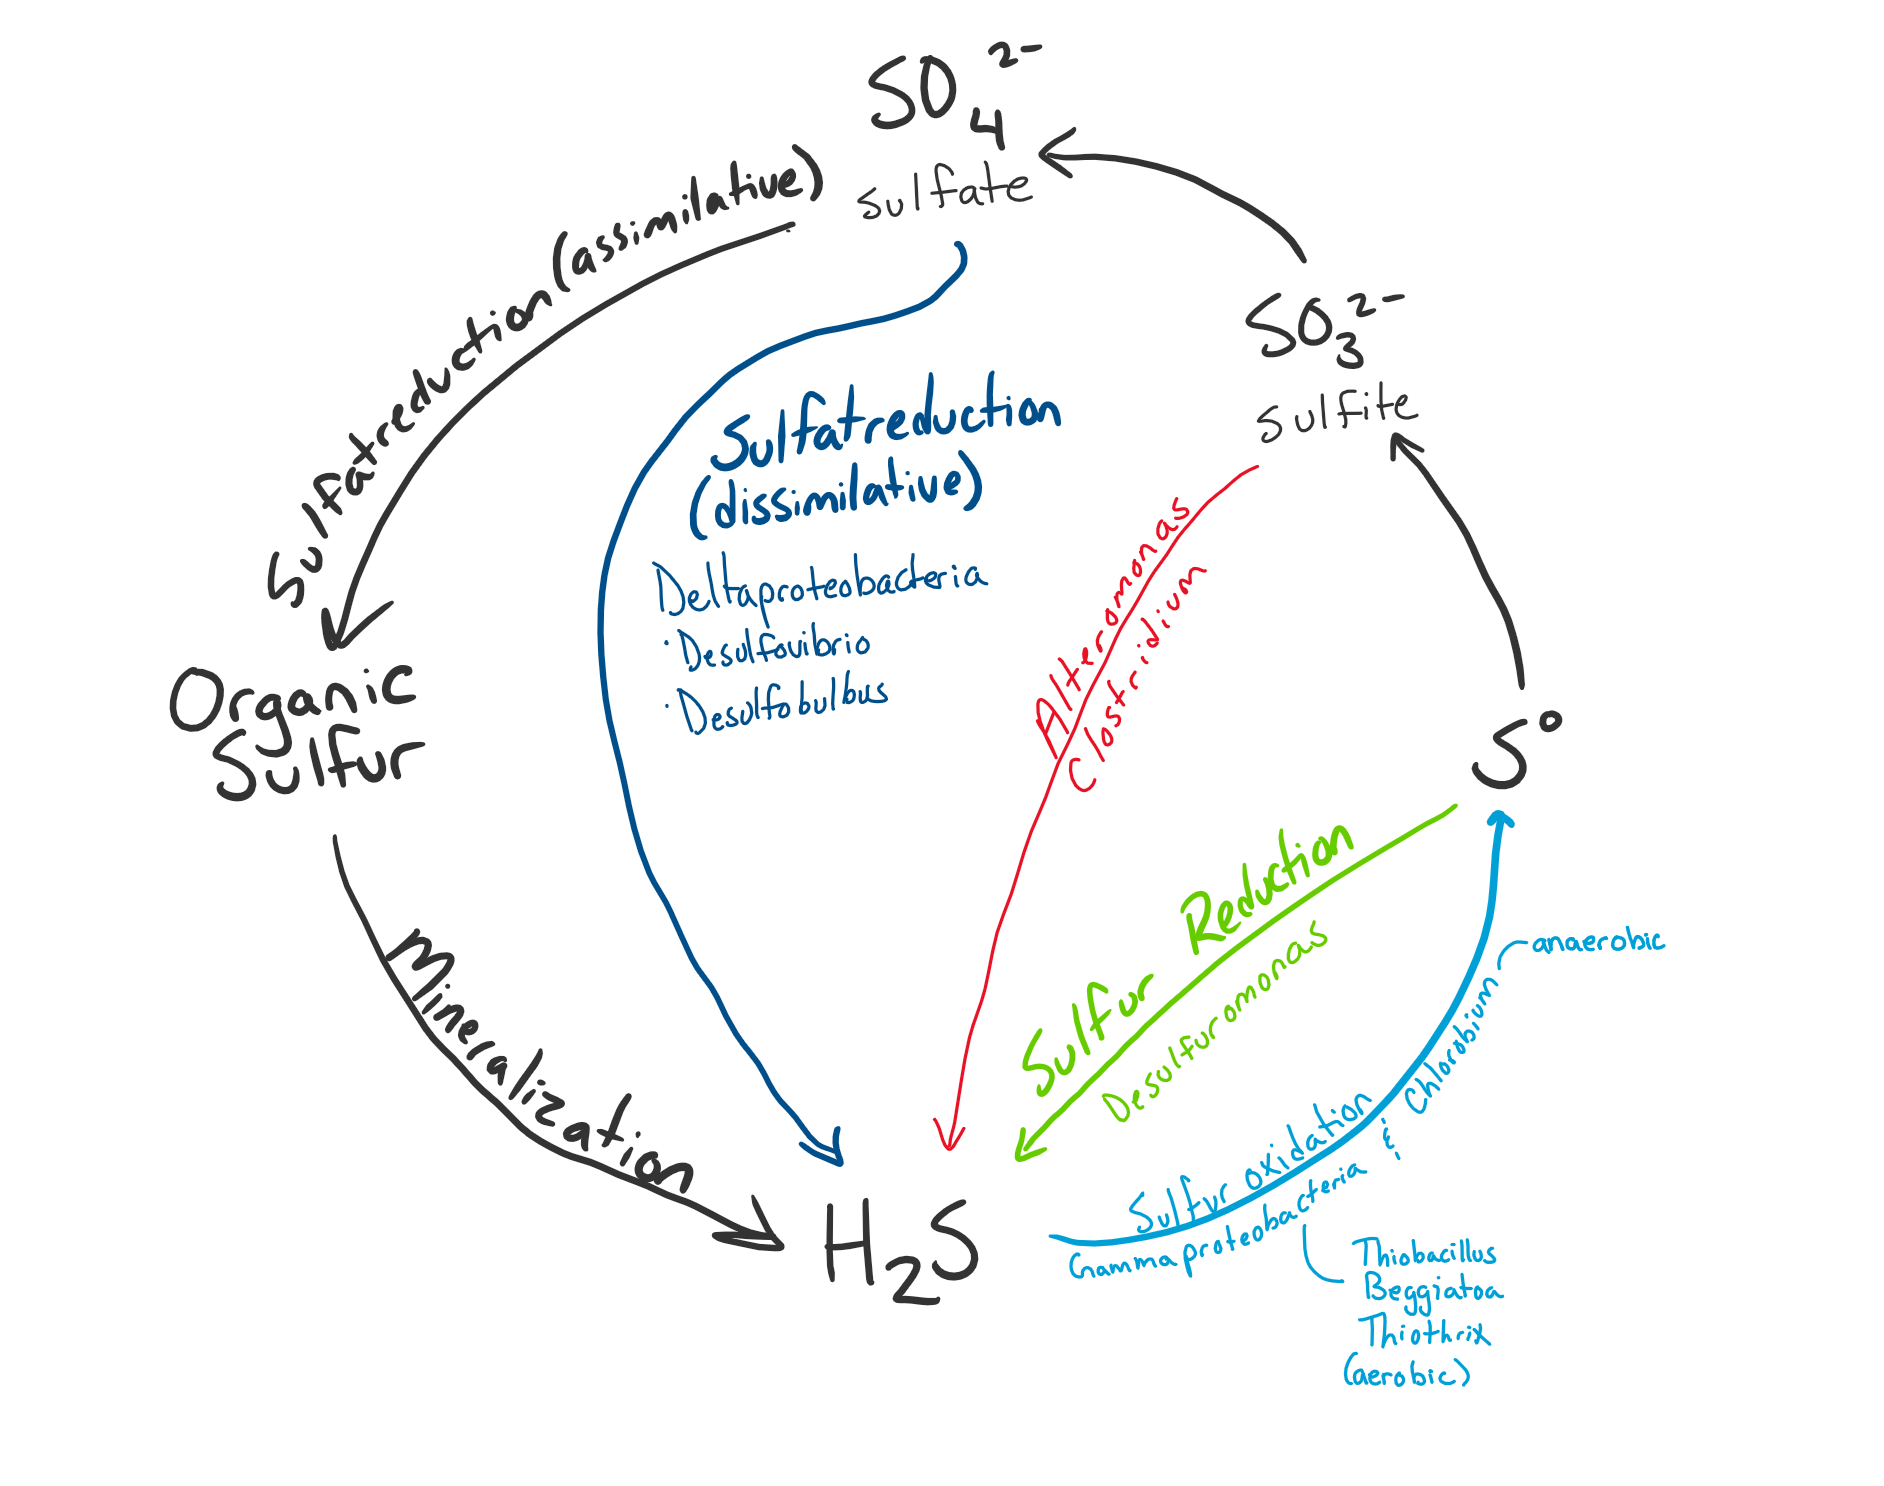
\includegraphics[width=0.65\textwidth]{figures/Sulfur_Cycle_for_Hydrothermal_Vents.png}
      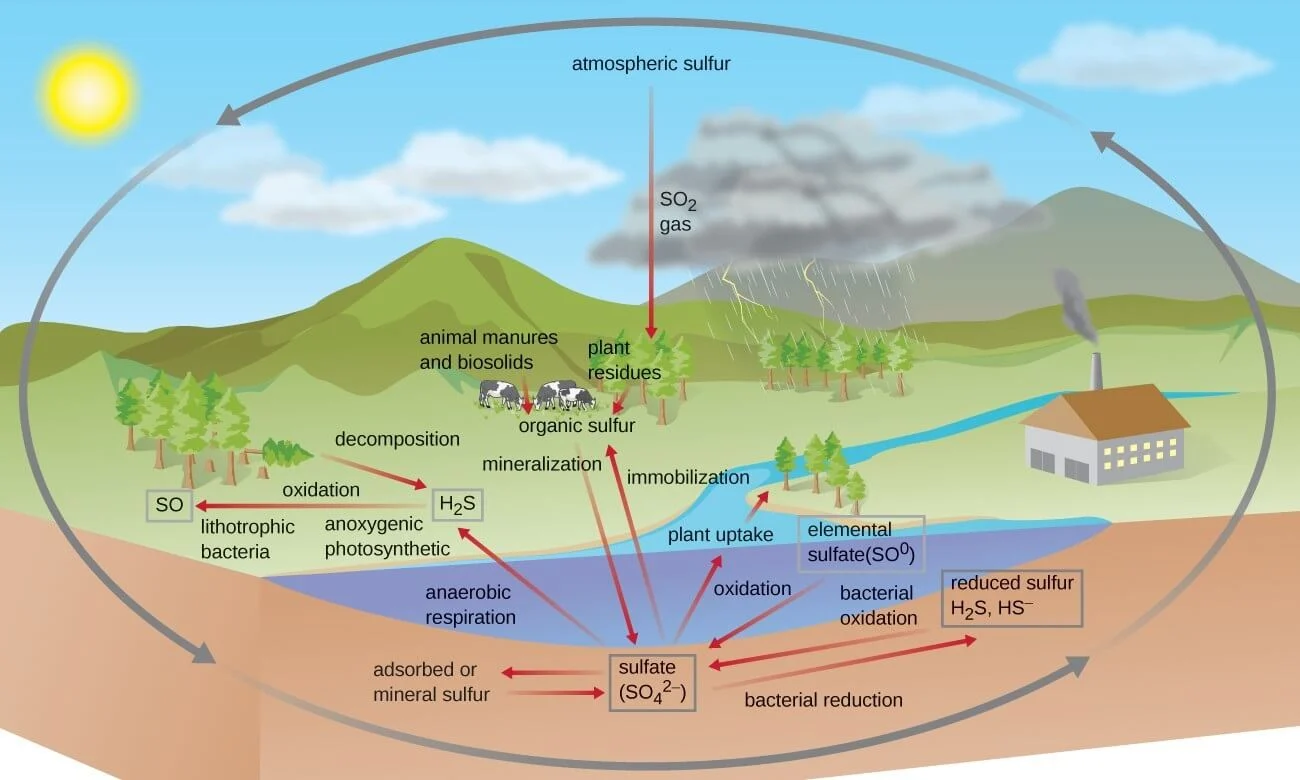
\includegraphics[width=0.95\textwidth]{figures/sulfur_village.png}
      \caption[The cycle of S and the role of microbial communiites]{
         The cycle of sulfur (S) (up) and the contribution of microbial communities on it (down, image source: \href{https://openstax.org/resources/3002d0fba25221d24455917117482a079a11f321}{OpenStax}).
         % Marine microbial communities contribute to CO$_2$ sequestration, nutrients recycle and thus to the release of CO$_2$ to the atmosphere. 
         % Soil microbial communities decomposers organic matter and release nutrients in the soil 
         % from \citep{cavicchioli2019scientists} doi: \href{https://doi.org/10.1038/s41579-019-0222-5}{10.1038/s41579-019-0222-5}, under \href{http://creativecommons.org/licenses/by/4.0 license}{Creative Commons Attribution 4.0 International License}
      }
      \label{fig:co2}
   \end{figure}

   The biological fluxes of most of the major elements (i.e., carbon, hydrogen, oxygen, nitrogen and sulfur) required
   for any biological macromolecule,
   are driven largely
   by microbially catalyzed, thermodynamically constrained redox reactions~\cite{falkowski2008microbial}. 
   Phosphorus the last of the 6 fundamental elements for life, is also included in the metabolic pathways catalyzed by microbes. 
   Thus, microbial communities consist of hundreds or even thousands of metabolically diverse strains and species~\cite{leventhal2018strain},
   and their functions
   and determine the fitness of most organisms on Earth. 
   In case of human health, specific microbial enzymatic pathways and molecules necessary for health promotion have been well known.
   Some of these "beneficial factors" are already known for probiotics and species in the human microbiome~\cite{marco2021defining}.


   % MICROBIAL ECOLOGY and OPEN QUESTIONS 
   % \if 0
   \subsection{The field of Microbial Ecology}
   % \fi
   Microbial ecology studies the interactions: 
   \begin{itemize}
      \setlength\itemsep{0.05em}
      \item between microbial taxa and their environment
      \item among the various microbial taxa present in a community, and
      \item between microbial taxa and their host~\cite{isme}
   \end{itemize}

   Microbial ecologists also investigate the role of microbial taxa in 
   biogeochemical cycles~\cite{falkowski2008microbial} and their interaction 
   with anthropogenic effects e.g. pollution and climate change~\cite{cavicchioli2019scientists}.

   Even though HTS has allowed a massive extension of our knowledge in  
   specific enzymatic reactions that regulate these pathways the rules that determine 
   the assembly, function, and evolution of these microbial communities remain unclear. 
   Thus, both in case of environmental and human
   the underlying mechanisms for how microbial assemblages work and affect their environment, remain to be discovered.
   Understanding the underlying governing principles is central to microbial ecology~\cite{giri2021metabolic} and crucial for designing microbial consortia for biotechnological~\cite{giri2020harnessing} or medical applications~\cite{kong2018designing}.

   Studies such as the one of~\citeauthor{louca2016decoupling}
   have opened new frontiers in our understanding on microbial assemblages. 
   After building metabolic functional groups and assigning more than 30,000 marine 
   species to these groups,~\citeauthor{louca2016decoupling} showed 
   that the distribution of these functional groups were influenced by environmental 
   conditions to a great extent, shaping \textit{metabolic niches}.
   At the same time though, the taxonomic composition within individual functional groups
   were not affected by such environmental condintions~\cite{louca2016decoupling}.

   % MICROBIAL INTERACTIONS INTRO
   % \if 0
   \subsection{Ecological interactions in microbial communities}
   % \fi
   Moreover, to elucidate how these assemblages work the biotic interactions have to be 
   considered too. 
   Microbial interactions play a fundamental role in deciphering the underlying mechanisms that govern ecosystem functioning \cite{braga2016microbial, faust2012microbial}. 
   Microbes secrete costly metabolites (called \textbf{byproducts}) to their environment, 
   which other microbes can absorb and exploit~\cite{pacheco2019costless}.
   By exchanging metabolic products, mostly as there are also other ways of interactions 
   e.g. quorum sensing, microbial taxa establish various interactions. 
   
   The interaction between two taxa can either be nutral or 
   positive / negative.
   In case of a positive interaction, 
   there is a case where both taxa benefit one from another.
   This \textit{win-win} relationship is called \textbf{mutualism} (or "cooperation")
   and it can be a result of
   \textit{cross-feeding}, in which two species exchange metabolic products~\cite{faust2012microbial}.
   Such is the case in biofilms where multiple bacterial taxa are working together  
   building a structure that provides them antibiotic resistance~\cite{santos2019evolutionary}.
   There is also the case where only one of the two taxa
   benefits without helping or harming the other; 
   this interaction is called \textbf{commensalism}~\cite{faust2012microbial}. 
   For example, \textit{Nitrosomonas} oxidize ammonia (NH$_3$) into nitrite (NO${_2}^{-}$), so  
   \textit{Nitrobacter} can use it to obtain energy and oxidize it into nitrate (NO${_3}^{-}$)~\cite{laanbroek2002nitrite}.
   Such interactions are quite common in microbial communities.

   \begin{figure}
      \centering
      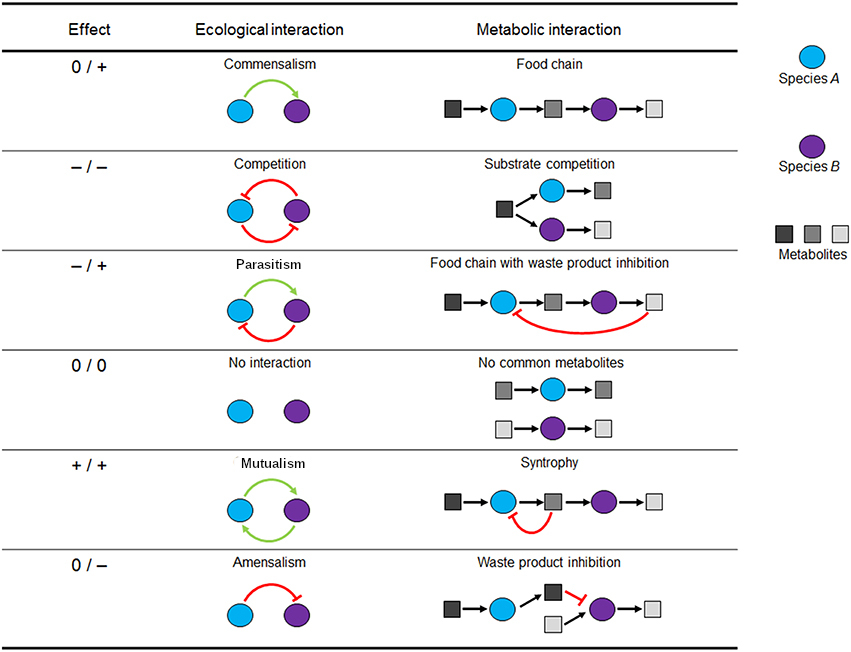
\includegraphics[width=.9\textwidth]{figures/interaction_types.jpg}
      \caption[Microbial interactions types]{Microbial interaction types along 
      with their corresponding metabolic ones.
      Due to certain metabolic interactions, two taxa may have a positive, a negative
      or a nutral effect one another. 
      Figure based on \cite{perez2016metabolic}}
      \label{fig:micro-inter-types}
   \end{figure}

   In case of a negative interaction, can harm each other either way (\textbf{compe-tition}). 
   That is the case between 
   \textit{Listeria monocytogenes} and \textit{Lactococcus lactis} in the study of~\citeauthor{freilich2010large} where their resource competition is high enough
   contributing to their non-overlapping existence~\cite{freilich2010large}.
   Moreover, similarly to commensalism, 
   there is also the case when a taxon has a negative affect on the other
   without getting any harm (\textbf{amensalism}). 
   Such is the case for \textit{Acidithiobacillus thiooxidant} that produces
   sulfuric acid (H$_2$SO$_4$) by oxidation of sulfur~\cite{bobadilla2013stoichiometric} which is responsible for lowering of pH in the culture media which inhibits the growth of most other bacteria~\cite{jin2018ph}.
   Finally, one of the taxa may have a positive affect (host) on the other, but the 
   latter (parasite) can be harmful to its benefator (\textbf{parasitism})~\cite{faust2012microbial}. 
   There are multiple cases of parasitism in real-world communities; 
   specis of the genus \textit{Bdellovibrio} for example, are parasites of other (gram-negative) bacteria~\cite{stolp1979interactions}.

   Apparently, the environmental conditions affect the ecological interactinos to a
   great extent. 
   A pair of taxa may be competitors in one case but have a nutral intrection in another one. 
   In addition, evolutionary processes may change certain interactions; 
   for example moving from commensalism to parasitism~\cite{parmentier2016commensalism}.
   Both ecological and environmental interactions 
   play a part in the composition and the functional potential of 
   microbial assemblages. 







% SECTION 2

\section{High Throughput Sequencing in Microbial Ecology}

      % SUBSECTION 1.1.2 
      \subsection{'Omics methods to access the \textit{who} and the \textit{what}}

      To discover the microbial taxa present in a sample, scientists have 
      explored multiple ways throught the years. 
      Only a particularly limited proportion of the microbial species 
      can be cultured~\cite{steen2019high}.
      Therefore, monocultures and enrichment cultures allow us to observe 
      only a small fraction of the actual diversity. 
      As a consequence, other methods for the taxonomic identification of theses
      species are required.
      Based on molecular characteristics of the microbial taxa, 
      over the last decades, a series of methods have been developed. 
 
      Moving from single species to assemblages, molecular-based identification and functional 
      profiling of communities has become available through marker (metabarcoding), 
      genome (metagenomics), or transcriptome (metatranscriptomics) sequencing from environmental 
      samples \citep{goldford2018emergent}. 
      To a great extent, these methods address the problem of how to produce and get access 
      to the information on different biological systems and molecules.

      In case that the taxonomic assesment of a sample is the aim of a study, 
      \textit{metabarcoding} (amplicon-targeted metagenomics) and \textit{shotgun metagenomics} can be used as alternative options. 
      Metabarcoding studies are common, well-established, cheaper and less computationally demanding than shotgun metagenomics~\cite{bell2021comparing}. 
      Its primary drawbacks are the limited information present in the short barcoding sequence and the possible taxonomic bias arising from differential efficiency of PCR primer pairing in different species~\cite{blazewicz2013evaluating}. 
      On the other hand, shotgun metagenomics offers a better taxonomic resolution at the species level by obtaining information from random sampling of virtually all genomic regions, and can address microbiome metabolic functions and entire biochemical pathways~\cite{sharpton2014introduction}. 
      Unfortunately, it requires higher sequencing coverage and, consequently, more complex and demanding downstream bioinformatic analysis~\cite{laudadio2018quantitative}. 
      Nevertheless, it has recently been suggested that shotgun metagenomics provides a deeper characterisation of microbiome complexity that metabarcoding recently enabling to profile up to the level of strains, whose non-core genome is responsible for crucial functional differences within the same species, as the fundamental units of the community~\cite{davila2019review, clooney2016comparing, segata2018road}.       
      
      The increasing performance of nucleic acid sequencing platforms at ever lower costs has allowed them to produce an unprecedented amount of data. 
      Targeting community composition and interaction in several ecological niches with no prior knowledge of the resident species, microbial ecologists produce vast 
      amount of sequencing data 
      while at the same time a number of challenges for their management and bioinformatics analysis is rising. 

      
      \subsection{Bioinformatics challenges in the analysis \& management of HTS data}

      Moving from raw data to taxonomic and functional profiles of a microbial community comes with high computational costs, especially in the case of metagenome studies~\cite{yang2021review}.
      Sequence pre-processing, assembly, classification, and functional annotation consist of several steps the most of which a significant number of algorithms or/and software tools are available~\cite{breitwieser2019review, roumpeka2017review}. 
      Tailoring each tool's execution parameters to reflect each experiment's idiosyncrasy is vital for legitimate findings, yet it makes analyses of metagenomic data even more complex. 
      The vast amounts of data that come with metagenomic studies and the computational complexity for implementing multiple steps mentioned earlier imply immense computational requirements for their analysis. 
      % Indicatively, the raw data of a metagenomic research may range from tens to hundreds of GB while the memory (RAM) required can exceed the order of hundreds of GB. 
      % At the same time, most of these steps are CPU - intensive jobs making the need for computing resources even more significant. 
      Therefore, several pipelines were 
      established to address the challenges of the bioinformatics analysis of metagenomes. 
      In addition, as such analyses exceed the capacity of a standard personal computer, computing infrastructures have been widely used to meet their needs. 
      Computing infrastructures may range from a local server of an individual lab to High-Performance Computing (HPC) or/and cloud solutions adopted at the (inter)national level, such as the \href{https://eosc-portal.eu}{EOSC} and 
      \href{https://www.embassycloud.org}{EMBL-EBI Embassy Cloud}. 

      The swift pace of establishing new algorithms and software as well as new versions of already published ones makes software versioning an essential issue for FAIR microbiome bioinformatics analyses. 


      By encapsulating all software and its dependencies in an isolated and easy to reinstall environment (container) containerization addresses this challenge. In addition, packaging a software per container simplifies management of the software requirements but also facilitates the creation and management of standardized workflows/pipelines. Workflow tools such as 
      \href{https://github.com/common-workflow-language/common-workflow-language}{Common Workflow Language (CWL)}, 
      \href{https://snakemake.github.io}{Snakemake} and \href{https://www.nextflow.io}{Nextflow} have been proven of high value in building such pipelines as they support the connection of multiple independent software.
      Another route of access to metagenomics analysis datasets is the Metagenome Exchange Registry which contains mappings between a number of well-established metagenome analysis platforms and their raw data in INSDC. Its aim is to aid comparison and benchmarking of tools and services as well as to help users explore metagenomics data in INSDC that are analysed by third party services. The registry is available as an API with plans to release a user interface in future.




      Challenges specific to metagenomic data further extend to complexities surrounding correctly labelling data that are biome-level and not representing a single species. For example, errors can be observed during taxonomic classification of metagenomic samples. Samples registered via one of the INSDC partners, must be assigned with a taxon from the NCBI taxonomy database and it is advised that metagenomic samples should use a taxon under the tax node metagenomes. Usage of a metagenomic taxon is important to distinguish environmental samples vs genomic samples. For example, the use of human gut metagenome (taxid: 408170) rather than Homo sapiens (taxid: 9606) for human gut samples immediately distinguishes a metagenomic sample derived from the human gut compared to a human genomic sample. However, users can understandably misdefine their taxonomic assignment for metagenomics data and label their samples after the host species if they are not aware of existing guidelines. This then has a knock-on effect on raw data retrieval where users searching for metagenomic data may miss out on a number of relevant datasets which are incorrectly defined. 

















\section{Systems Biology: data integration in the service of microbial ecology}


   \subsection*{Metadata: a key issue for the microbiome community}

      The Community initially focused on developing open science "best practices" for the research community. 
      The paper "The metagenomic data life-cycle: standards and best practices" \citep{ten2017metagenomic} provided the foundation for FAIR data management in the domain. 
      These best practices advocated using community standards for contextual provenance and metadata at all stages of the research data life cycle.

      Alongside archived sequence data, access to comprehensive metadata is important to contextualise where the data originated. 
      On submission, submitters are given the option to provide details regarding when, where and how their samples were collected with the opportunity to align provided metadata against community developed standards where possible. 
      However, challenges associated with metadata deposition mean submitters do not always provide comprehensive metadata - these challenges can range from: 
      lack of training and outreach resulting in submitters not fully understanding the importance of metadata and how to comply with standards; 
      as well as the trade-offs for the archives to provide complex and thorough validation vs simple user interfaces to ensure both compliance and submission are as easy as possible. 
      For the ENA, extensive documentation exists on how to submit data which both encourages compliance with metadata standards and provides separate submission guidelines for different data types - usage of the documentation can mitigate common errors and often aid first-time submitters but does not reach the full user-base. 

      FAIR principles, to provide a multilayer set of metadata required by the different scientific communities, reflecting the inherently multi-disciplinary character of environmental microbiology. 
      The various layers of metadata necessary for the FAIRification of MAGs should include:
      \begin{enumerate}
         \item Environmental data describing the sample of origin
         \item Sequencing technology or technologies
         \item Details on the computational pipeline for metagenome assembly, binning and quality assessment
         \item Connection to an existing taxonomy schema
      \end{enumerate}


      OSD’s open access strategy and provenance for metadata annotation is reflected in its ENA and Pangea submissions. 
      Among others Standardization and training are key aspects across OSD: from sampling protocols to metadata checklists and guidelines. 
      This is inline with aims of the Elixir microbiome community (see Sections "Mobilising raw data and metadata", 
      "Training - lack of training"); 
      spreading the experience to other biomes can benefit such ends.


      Open questions: 
      Metadata standard definition: minimum set and formats (Some flexibility will have to be considered in sharing standards between domain-specific communities).
      Systems to extract the vast amount of metadata locked in the scientific literature and provide them in standard format (explored by the Biodiversity Focus Group).


      Metadata associated with the raw data, the assembled data, and the workflow. The necessary scripts will be written in Python using standard libraries and Biopython. 
      Metadata of the cleaned data
      Metadata associated with the data sequencing, sample collection (MIMS), and quality control analyses will be generated according to the ENA manifest to enable uploading and archiving of the data to ENA.
      Metadata of the assembled data
      Because the workflow is distributed, it is necessary for EBI-MGnify to verify the provenance of the data workflow through registration and a verification test. A unique calculated hash generated from the data and workflow code will serve as a key for verification. This metadata will be generated at this step and together with the metadata associated with the assembly, uploaded to ENA/MGnify for further downstream functional annotation.
      Metadata to accompany the taxonomic inventories
      Metadata associated with the previous two steps will be summarised for inclusion with the taxonomic inventories (biom file format and CSV) for publication on the EMBRC GOs website.


      \begin{itemize}
         \item Metadata of the cleaned data; metadata associated with the data sequencing, sample collection (MIMS), and quality control analyses
         \item Metadata of the assembled data
         \item Metadata to accompany the taxonomic inventories

      \end{itemize}  




   \subsection*{Ontologies \& databases: the corner stone of mordern biology}


      Databases

      \begin{itemize}
         \item GenBank, ENA
         \item repositories such as MGnify 
         \item PubMed
      \end{itemize}


      Ontologies: 

      \begin{itemize}
         \item ENVO
         \item NCBI Taxonomy 
         \item Gene Ontology 
         \item Uniprot
         \item KEGG
         \item https://edamontology.org/page
      \end{itemize}



\section{Reverse ecology: transforming ecology into a high-throughput field}


   % - genotype - phenotype relationship \\
   Chapter 15
   Reverse Ecology: From Systems
   to Environments and Back


   (from Roie Levy and Elhanan Borenstein~\cite{levy2012reverse})
   Reverse Ecology—an emerging new frontier in Evolutionary Systems Biology—aims
   to extract this information and to obtain novel insights into an organism’s ecology.
   The Reverse Ecology framework facilitates the translation of high-throughput
   genomic data into large-scale ecological data, and has the potential to transform
   ecology into a high-throughput field


   the traditional approach taken to studies relating genetics and ecology:
   first an ecological adaptive phenotype is identified, then various methodologies are
   employed to detect causal genetic variation.






   In some cases, however, one may wish to predict not only potential interactions
   but also specific metabolic dynamics in a community of microorganisms and the
   exact set of metabolites being exchanged actively between the various species. The
   prediction of specific metabolic fluxes is mostly beyond the scope of topology-
   based metabolic models and requires a more involved modeling framework such
   as constraint-based modeling (CBM) [18, 19]. Such models, however, are usually
   limited in scale and require detailed and manually curated data [20].







   (from RevEcoR publication~\cite{cao2016revecor})
   A systematic approach for describing microbiome ecologies and the interactions between microbiota is lacking. 
   To address this challenge, a systems biology approach called \textit{reverse ecology} has been developed 
   to study the complex interactions and species composition of microbial communities [4]. 
   Reverse ecology uses genomics to study community ecology with no a priori assumptions about the organisms under consideration. 
   Researchers can use it to infer the ecology of a system directly from genomic information. 
   The reverse ecology framework uses advances in systems biology and genomic metabolic modeling and 
   the system-level analysis of complex biological networks to predict the ecological traits of poorly studied microorganisms, 
   their interactions with other microorganisms, and the ecology of microbial communities. 
   Several studies have applied this approach to investigate the interactions between microorganisms 
   and their surroundings on a large scale [4, 5].

   The relationship between genotype and phenotype is fundamental to biology.
   Many levels of control are introduced when moving from one to the other. 
   Systems biology aims at deciphering "the strategy" both at the cell and at higher levels of organization, in case of multicell species, that enables organisms to produce orderly adaptive behavior in the face of widely varying genetic and environmental conditions (\cite{strohman2002maneuvering}); 
   the term "strategy" is used as per \cite{polanyi1968life}.
   Systems biology approaches aim at interpreting how a system's properties emerge; 
   from the cell to the community level.
   As \citeauthor{polanyi1968life} (\citeyear{polanyi1968life}) underlines 
   "live mechanisms and information in DNA are boundary conditions with a sequence of boundaries above them". 

   \begin{figure}[h]
      \centering
      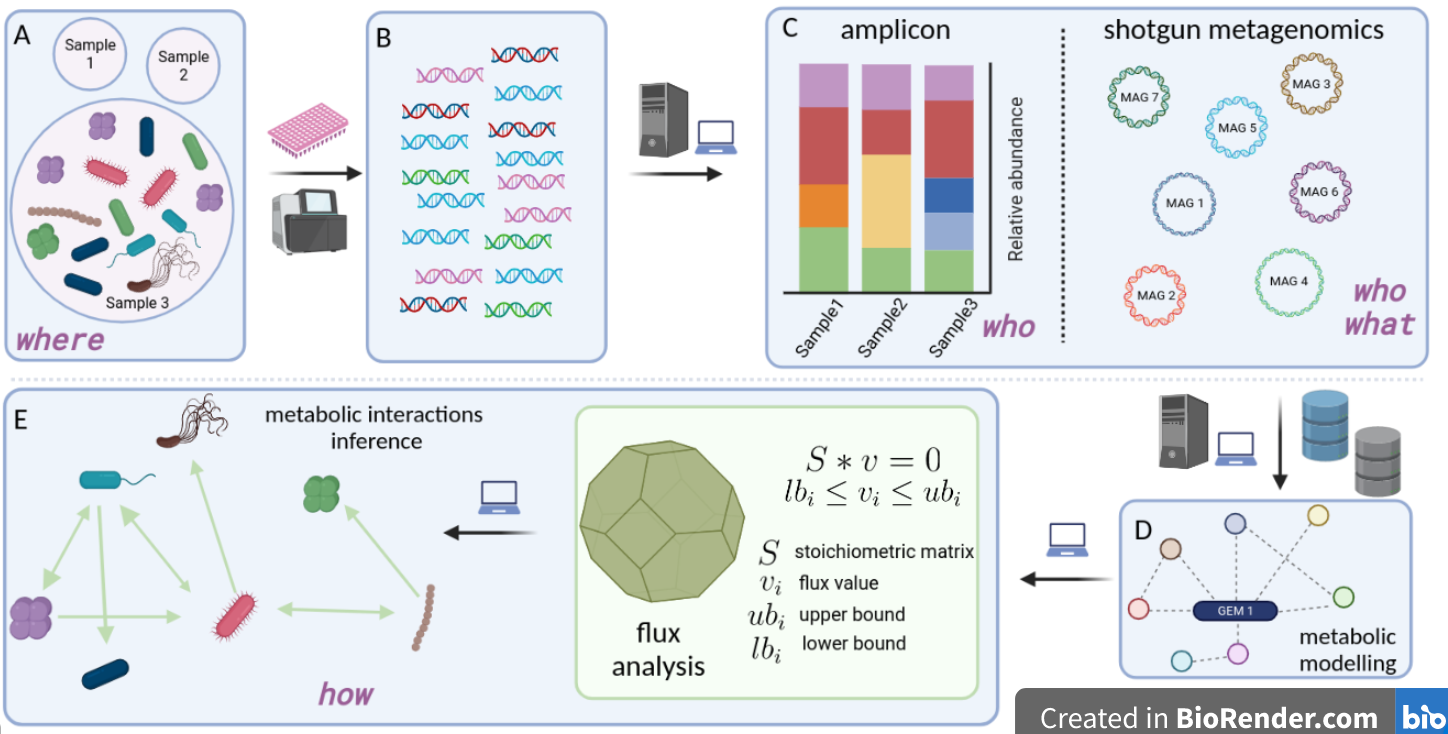
\includegraphics[width=135mm]{figures/Selection_935.png}
      \caption[Reverse ecology approach]{}
   \end{figure}



% SECTION 4
\section{Metabolic networks: modeling  cellular physiology and growth}
   % SUBSECTION FOR THE REVERSE ECOLOGY FRAMEWORK


% 
   \subsection*{Genome-scale metabolic model analysis}



      Being at the helm of the most critical celular functions, 
      metabolism and therefore, metabolic networks and their analysis, 
      play a key role in Systems Biology. 
      Moreover, \citeauthor{lewis2012constraining} (\citeyear{lewis2012constraining}) 
      describe thoroughly the multiple constraint-based reconstruction and analysis (COBRA) methods 
      that have been developed to support the analysis of such networks. 
   \subsection*{Sampling the flux space of a metabolic model: challenges \& potential}





% SECTION 7 - first draft ready
\section{Aims and objectives}

   The aim of this PhD was double:
   \begin{enumerate}
      \item to enhance the analysis of microbiome data by building algorithms and software 
            to address some of the on-going computational challenges on the field.
      \item to exploit these methods to identify taxa, functions, especially related to sulfur cycle, 
            and microbial interactions that support life in microbial community assemblages in hypersaline sediments.
   \end{enumerate}
   All parts of this work are purely computational. 
   Samples and their corresponding sequencing data used in Chapter~\ref{cha:swamp} have been collected 
   and produced by \href{https://scholar.google.com/citations?user=3zs1rNkAAAAJ&hl=en&oi=sra}{Dr. Christina Pavloudi}. 

   In \textbf{Chapter~\ref{cha:2}}, challenges derived from the analysis of HTS amplicon data are examined.
   A bioinformatics pipeline, called \texttt{pema}, for the analysis of several marker genes was developed, combinining several new technologies that allow large scale analysis of hundreds of samples. 
   In addition, a software tool called \texttt{darn}, was built to investigate the unassigned sequences in amplicon data of the COI marker gene. 

   In \textbf{Chapter~\ref{cha:swamp}}, sediment samples from a hypersaline swamp in Tristomo, Karpathos Greece were analysed using both amplicon and shotgun metagenomics. 
   The taxonomic and the functional profiles of the microbial communities present there were investigated. 
   Key metabolic processes for ensuring life at such an extreme environment were identified.
   Microbial interactions of the assemblages retrieved were also studied. 

   In \textbf{Chapter~\ref{cha:prego}}, data integration, data mining and text-mining methods were exploited to build a knowledge-base, called \texttt{prego}, including millions of associations between:
   \begin{enumerate}
      \item microbial taxa and the environments they have been found in 
      \item microbial taxa and biological processes they occur
      \item environmental types and the biological processes that take place there
   \end{enumerate}

   In \textbf{Chapter~\ref{cha:dingo}}, the challenges of flux sampling in metabolic models of high dimensions was presented along with a Multiphase Monte Carlo Sampling (MMCS) algorithm we developed. 

   In \textbf{Chapter~\ref{cha:hpc}}, the history of the IMBBC-HCMR HPC facility was presented indicating the vast needs of computing resources in modern analyses in general and in microbial studies more specifically. 


   Finally, in \textbf{Chapter~\ref{cha:conclusion}}, general discussion and conclusions that have derived from this research were presented. 





% -------------------------
%    NOTES
% -------------------------
% 
%    biotic interactions                  --> cross-feeding of byproduscts, competition for nutrients 
%    confounder (or 'confounding factor') --> something, other than the thing being studied, that could be causing the results seen in a study. 
%                                             confounders have the potential to change the results of research because they can influence the outcomes
%                                             that the researchers are measuring.
%                                             EXAMPLE: we found that people eating red meat have higher possibility for heart issues; but we have to 
%                                                      check whether everyone in the study who ate a lot of red meat may also have smoked cigarettes
%                                                      regularly or been overweight. 
%    circumvented                         --> shortchut, find a way around (an obstacle).
%    stratify                             --> stromatopoio // 
%    stringent                            --> austiros, strict
%    a habitat filtering model supposes that
% habitats with differing environmental
% features support non-overlapping sets of taxa
